\documentclass[border=12pt]{standalone}
\usepackage[dvipsnames]{xcolor}
\usepackage{pifont,amsmath}
\usepackage{tikz}
\usetikzlibrary{arrows.meta, positioning, calc, shadows, decorations.pathreplacing, shapes.geometric}

\definecolor{gold}{HTML}{CFB87C}
\definecolor{dkblue}{HTML}{156082}
\definecolor{accent2}{HTML}{E97132}
\definecolor{accent3}{HTML}{196B24}
\definecolor{dkgray}{HTML}{333333}
\definecolor{medgray}{HTML}{888888}
\definecolor{dkred}{HTML}{C0392B}
\definecolor{ltred}{HTML}{FDE8E8}
\definecolor{ltgreen}{HTML}{E8F5E9}
\definecolor{cardbg}{HTML}{FAFAF7}

\begin{document}
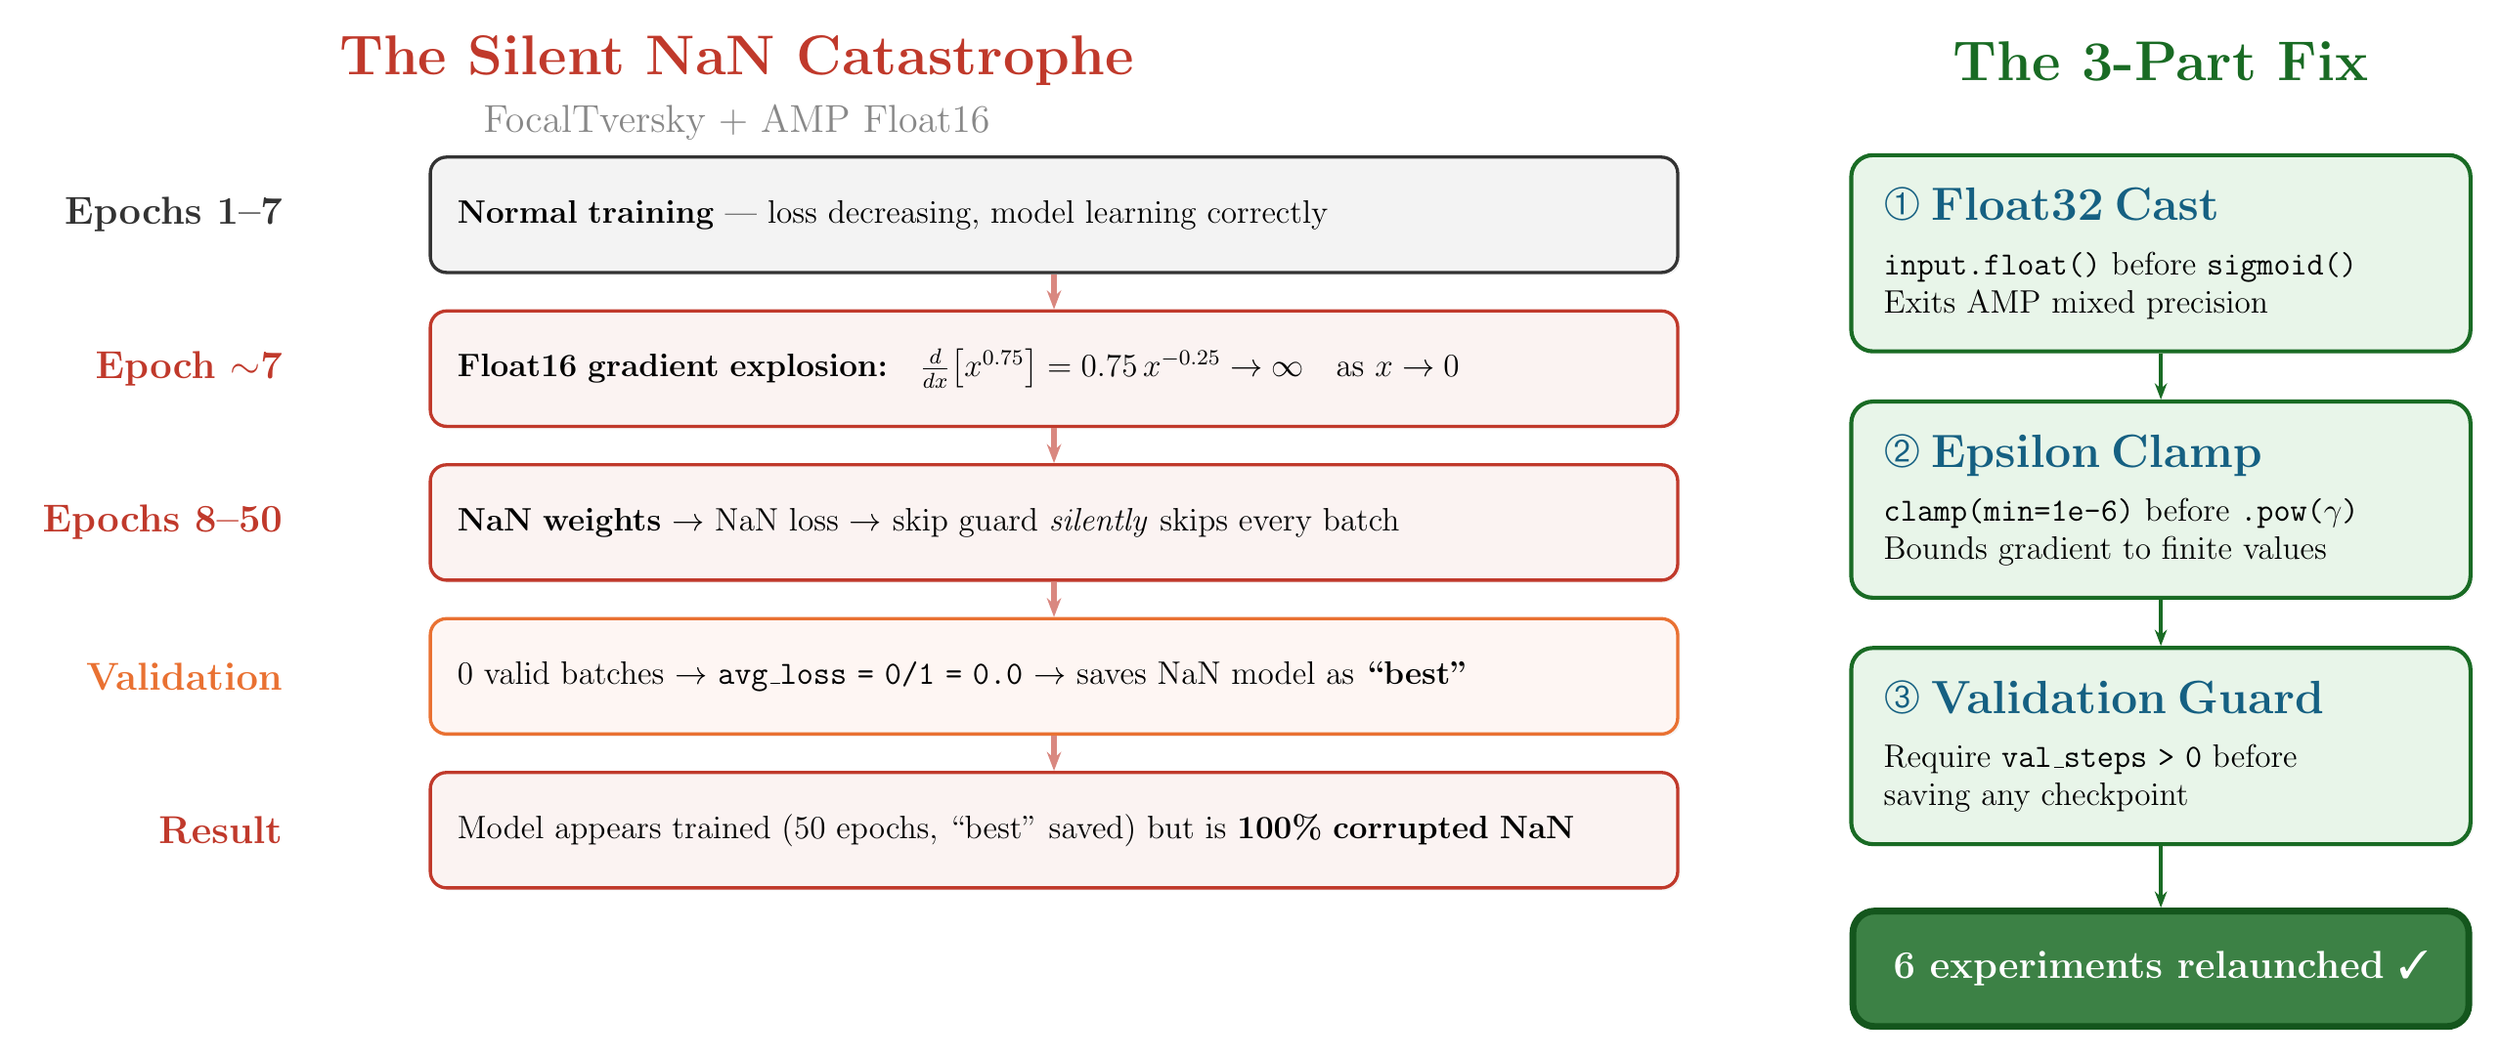
\begin{tikzpicture}[
    node distance=0.6cm,
    event/.style={
        draw=#1, fill=#1!6, rounded corners=6pt,
        line width=1.2pt, minimum width=16cm, minimum height=1.5cm,
        text width=15.5cm, align=left, font=\large, inner sep=10pt,
        drop shadow={shadow xshift=1pt, shadow yshift=-1pt, opacity=0.08}
    },
    tlabel/.style={
        font=\Large\bfseries, color=#1, text width=3.2cm, align=right
    },
    fixcard/.style={
        draw=accent3, fill=ltgreen, rounded corners=8pt,
        line width=1.5pt, minimum width=8cm, minimum height=2.2cm,
        text width=7.2cm, align=left, font=\large, inner sep=12pt,
        drop shadow={shadow xshift=1pt, shadow yshift=-1pt, opacity=0.08}
    },
    >=Stealth
]

% ===== LEFT SIDE: NaN Cascade =====
\node[font=\huge\bfseries, color=dkred] at (6.5, 1.5) {The Silent NaN Catastrophe};
\node[font=\Large\color{medgray}] at (6.5, 0.7) {FocalTversky + AMP Float16};

% Timeline events
\node[tlabel=dkgray] (t1) at (-1, -0.5) {Epochs 1--7};
\node[event=dkgray, anchor=west] (e1) at (2.5, -0.5) {%
    \textbf{Normal training} --- loss decreasing, model learning correctly%
};

\node[tlabel=dkred] (t2) at (-1, -2.5) {Epoch $\sim$7};
\node[event=dkred, anchor=west] (e2) at (2.5, -2.5) {%
    \textbf{Float16 gradient explosion:}\quad
    $\frac{d}{dx}\bigl[x^{0.75}\bigr] = 0.75\,x^{-0.25} \to \infty$\quad as $x \to 0$%
};

\node[tlabel=dkred] (t3) at (-1, -4.5) {Epochs 8--50};
\node[event=dkred, anchor=west] (e3) at (2.5, -4.5) {%
    \textbf{NaN weights} $\to$ NaN loss $\to$ skip guard \emph{silently} skips every batch%
};

\node[tlabel=accent2] (t4) at (-1, -6.5) {Validation};
\node[event=accent2, anchor=west] (e4) at (2.5, -6.5) {%
    0 valid batches $\to$ \texttt{avg\_loss = 0/1 = 0.0} $\to$ saves NaN model as \textbf{``best''}%
};

\node[tlabel=dkred] (t5) at (-1, -8.5) {Result};
\node[event=dkred, anchor=west] (e5) at (2.5, -8.5) {%
    Model appears trained (50 epochs, ``best'' saved) but is \textbf{100\% corrupted NaN}%
};

% Cascade arrows — simple vertical connectors between boxes
\foreach \i/\j in {e1/e2, e2/e3, e3/e4, e4/e5} {
    \draw[-{Stealth[length=7pt]}, dkred!60, line width=2pt]
        (\i.south) -- (\j.north);
}

% ===== RIGHT SIDE: Fix =====
\node[font=\huge\bfseries, color=accent3] at (25, 1.5) {The 3-Part Fix};

\node[fixcard] (f1) at (25, -1) {%
    {\LARGE\bfseries\color{dkblue}\ding{192}\ Float32 Cast}\\[6pt]
    \texttt{input.float()} before \texttt{sigmoid()}\\
    Exits AMP mixed precision%
};

\node[fixcard, below=0.6cm of f1] (f2) {%
    {\LARGE\bfseries\color{dkblue}\ding{193}\ Epsilon Clamp}\\[6pt]
    \texttt{clamp(min=1e-6)} before \texttt{.pow($\gamma$)}\\
    Bounds gradient to finite values%
};

\node[fixcard, below=0.6cm of f2] (f3) {%
    {\LARGE\bfseries\color{dkblue}\ding{194}\ Validation Guard}\\[6pt]
    Require \texttt{val\_steps > 0} before\\
    saving any checkpoint%
};

% Result box — DARK green background with WHITE text (high contrast)
\node[draw=accent3!80!black, fill=accent3!85, rounded corners=8pt, line width=2.5pt,
      minimum width=8cm, minimum height=1.5cm, text width=7.2cm, align=center,
      font=\Large\bfseries, inner sep=10pt, below=0.8cm of f3,
      drop shadow={shadow xshift=1pt, shadow yshift=-1pt, opacity=0.10}]
    (fr) {\color{white} 6 experiments relaunched \ding{51}};

% Fix arrows
\draw[-{Stealth[length=6pt]}, accent3, line width=1.5pt] (f1.south) -- (f2.north);
\draw[-{Stealth[length=6pt]}, accent3, line width=1.5pt] (f2.south) -- (f3.north);
\draw[-{Stealth[length=6pt]}, accent3, line width=1.5pt] (f3.south) -- (fr.north);

\end{tikzpicture}
\end{document}
